\section*{BT ÔN TẬP HÀM SỐ - SỐ 2}
\setcounter{ex}{0}\setcounter{bt}{0}
\Opensolutionfile{ans}[ans/ansOC3-CD-1]

\begin{ex}%[Phan Anh]%[0D2K1-3]
    \immini{Cho đồ thị hàm số $y=x^3$ như hình bên. Khẳng định nào sau đây \textbf{sai}?
    \choice
    {Hàm số đồng biến trên khoảng $\left(-\infty;0\right)$}
    {Hàm số đồng biến trên khoảng $\left(0;+\infty \right)$}
    {Hàm số đồng biến trên khoảng $\left(-\infty;+\infty \right)$}
    {\True Hàm số đồng biến tại gốc tọa độ $O$}}
{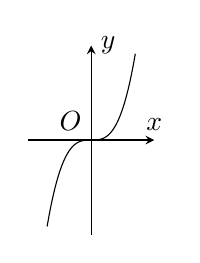
\begin{tikzpicture}[>=stealth,scale=0.4]
    \draw[->](-2,0)--(2,0)node[above]{$x$};
    \draw[->](0,-3)--(0,3)node[right]{$y$};
    \draw[smooth,samples=100,domain=-1.4:1.4]plot(\x,{(\x)^3});
    \fill (0,0)node[above left]{$O$}circle(1.2pt);
    \end{tikzpicture}}
    \loigiai{Dựa vào đồ thị, ta thấy hàm số đồng biến trên toàn miền xác định. Nhưng không thể đồng biến chỉ tại đúng một điểm.}
\end{ex}

\begin{ex}%[Phan Anh]%[0D2K1-3]
    Có bao nhiêu giá trị nguyên của tham số $m$ thuộc đoạn $\left[-3;3\right]$ để hàm số $f(x)=\left(m+1\right)x+m-2$ đồng biến trên $\mathbb{R}$?
    \choice
    {$7$}
    {$5$}
    {\True $4$}
    {$3$}
    \loigiai{
        Tập xác định $\mathscr{D}=\mathbb{R}.$\\
        Với mọi $x_1,x_2\in\mathscr{D}$ và $x_1<x_2$. \\Ta có
        $f\left(x_1\right)-f\left(x_2\right)=\left[\left(m+1\right)x_1+m-2\right]-\left[\left(m+1\right)x_2+m-2\right]=\left(m+1\right)\left(x_1-x_2\right).$\\
        Suy ra $\dfrac{f\left(x_1\right)-f\left(x_2\right)}{x_1-x_2}=m+1$.\\
        Để hàm số đồng biến trên $\mathbb{R}$ khi và chỉ khi
        $m+1>0\Leftrightarrow m>-1\xrightarrow{m\in \left[-3;3\right]}{m\in \mathbb{Z}}\Rightarrow m\in \left\{0;1;2;3\right\}$.\\
        Vậy có 4 giá trị nguyên của $m$ thỏa mãn.}
\end{ex}

\begin{ex}%[Phan Anh]%[0D2B1-2]
    Tìm tập xác định $\mathscr{D}$ của hàm số $y=\sqrt{\sqrt{x^2+2x+2}-(x+1)}$.
    \choice
    {$\mathscr{D}=\left(-\infty;-1\right)$}
    {$\mathscr{D}=\left[-1;+\infty \right)$}
    {$\mathscr{D}=\mathbb{R}\setminus\left\{-1\right\}$}
    {\True $\mathscr{D}=\mathbb{R}$}
    \loigiai{
        Hàm số xác định khi $\begin{aligned}[t]
        &\sqrt{x^2+2x+2}-(x+1)\ge 0\Leftrightarrow \sqrt{(x+1)^2+1}\ge x+1\\
        \Leftrightarrow&\, \hoac{
            & \heva{
                & x+1<0 \\ 
                & (x+1)^2+1\ge 0}\\ 
            & \heva{
                & x+1\ge 0 \\ 
                & (x+1)^2+1\ge(x+1)^2}}\Leftrightarrow \hoac{
            & x+1<0 \\ 
            & x+1\ge 0}\Leftrightarrow x\in \mathbb{R}.
        \end{aligned}$\\
        Vậy tập xác định của hàm số là $\mathscr{D}=\mathbb{R}$.}
\end{ex}

\begin{ex}%[Phan Anh]%[0D2K1-3]
    Tìm tất cả các giá trị thực của tham số $m$ để hàm số $y=-x^2+\left(m-1\right)x+2$ nghịch biến trên khoảng $\left(1;2\right)$.
    \choice
    {$m<5$}
    {$m>5$}
    {\True $m<3$}
    {$m>3$}
    \loigiai{
        Với mọi $x_1\ne x_2$, ta có\\
        $\dfrac{f\left(x_1\right)-f\left(x_2\right)}{x_1-x_2}=\dfrac{\left[-x_1^2+\left(m-1\right)x_1+2\right]-\left[-x_2^2+\left(m-1\right)x_2+2\right]}{x_1-x_2}=-\left(x_1+x_2\right)+m-1.$\\
        Để hàm số nghịch biến trên $\left(1;2\right)\Leftrightarrow-\left(x_1+x_2\right)+m-1<0$, với mọi $x_1,x_2\in \left(1;2\right)$\\
        $\Leftrightarrow m<\left(x_1+x_2\right)+1$, với mọi $x_1,x_2\in \left(1;2\right)$
        $\Leftrightarrow m<\left(1+1\right)+1=3$.}
\end{ex}

\begin{ex}%[Phan Anh]%[0D2K1-2]
    Tìm tập xác định $\mathscr{D}$ của hàm số $f(x)=\left\{\begin{array}{*{35}{l}}
    \dfrac{1}{x} &;x\ge 1 \\
    \sqrt{x+1} &;x<1.
    \end{array}\right.$
    \choice
    {$\mathscr{D}=\left\{-1\right\}$}
    {$\mathscr{D}=\mathbb{R}$}
    {\True $\mathscr{D}=\left[-1;+\infty \right)$}
    {$\mathscr{D}=\left[-1;1\right)$}
    \loigiai{
        Hàm số xác định khi $\hoac{
            & \heva{
                & x\ge 1 \\ 
                & x\ne 0} \\ 
            & \heva{
                & x<1 \\ 
                & x+1\ge 0}}\Leftrightarrow \hoac{
            & x\ge 1 \\ 
            & \heva{
                & x<1 \\ 
                & x\ge-1.}}$\\
        Vậy xác định của hàm số là $\mathscr{D}=\left[-1;+\infty \right)$.}
\end{ex}

\begin{ex}%[Phan Anh]%[0D2B1-4]
    Trong các hàm số nào sau đây, hàm số nào là hàm số chẵn?
    \choice
    {\True $y=\left| x+1\right|+\left| x-1\right|$}
    {$y=\left| x+3\right|+\left| x-2\right|$}
    {$y=2x^3-3x$}
    {$y=2x^4-3x^2+x$}
    \loigiai{
        Xét $f(x)=\left| x+1\right|+\left| x-1\right|$ có $\mathscr{D}=\mathbb{R}$ nên $\forall x\in\mathscr{D}\Rightarrow-x\in\mathscr{D}$.\\
        Ta có $f\left(-x\right)=\left|-x+1\right|+\left|-x-1\right|=\left| x-1\right|+\left| x+1\right|=f(x)\Rightarrow f(x)$ là hàm số chẵn.}
\end{ex}

\begin{ex}%[Phan Anh]%[0D2B1-2]
    Tìm tập xác định $\mathscr{D}$ của hàm số $y=\dfrac{\sqrt{3x-2}+6x}{\sqrt{4-3x}}$.
    \choice
    {\True $\mathscr{D}=\left[\dfrac{2}{3};\dfrac{4}{3}\right)$}
    {$\mathscr{D}=\left[\dfrac{3}{2};\dfrac{4}{3}\right)$}
    {$\mathscr{D}=\left[\dfrac{2}{3};\dfrac{3}{4}\right)$}
    {$\mathscr{D}=\left(-\infty;\dfrac{4}{3}\right)$}
    \loigiai{
        Hàm số xác định khi $\heva{
            & 3x-2\ge 0 \\ 
            & 4-3x>0}\Leftrightarrow \heva{
            & x\ge \dfrac{2}{3} \\ 
            & x<\dfrac{4}{3}}\Leftrightarrow \dfrac{2}{3}\le x<\dfrac{4}{3}$.\\
        Vậy tập xác định của hàm số là $\mathscr{D}=\left[\dfrac{2}{3};\dfrac{4}{3}\right)$.}
\end{ex}

\begin{ex}%[Phan Anh]%[0D2B1-2]
    Tìm tập xác định $\mathscr{D}$ của hàm số $y=\dfrac{2x-1}{(2x+1)(x-3)}$.
    \choice
    {$\mathscr{D}=(3;+\infty)$}
    {\True $\mathscr{D}=\mathbb{R}\setminus\left\{-\dfrac{1}{2};3\right\}$}
    {$\mathscr{D}=\left(-\dfrac{1}{2};+\infty\right)$}
    {$\mathscr{D}=\mathbb{R}$}
    \loigiai{
        Hàm số xác định khi $\heva{
            & 2x+1\ne 0 \\ 
            & x-3\ne 0}\Leftrightarrow \heva{
            & x\ne-\dfrac{1}{2} \\ 
            & x\ne 3.}$\\
        Vậy tập xác định của hàm số là $ \mathscr{D}=\mathbb{R}\setminus\left\{-\dfrac{1}{2};3\right\}$}
\end{ex}

\begin{ex}%[Phan Anh]%[0D2K1-2]
    Tìm tất cả các giá trị thực của tham số $m$ để hàm số $y=\sqrt{x-m}+\sqrt{2x-m-1}$ xác định trên $(0;+\infty)$.
    \choice
    {$m\le 0$}
    {$m\ge 1$}
    {$m\le 1$}
    {\True $m\le-1$}
    \loigiai{
        Hàm số xác định khi $\heva{
            & x-m\ge 0 \\ 
            & 2x-m-1\ge 0}\Leftrightarrow \heva{
            & x\ge m \\ 
            & x\ge \dfrac{m+1}{2}}\,(*)$.
        \begin{itemize}
            \item Nếu $m\ge \dfrac{m+1}{2}\Leftrightarrow m\ge 1$ thì $\left(*\right)\Leftrightarrow x\ge m$.\\
            Tập xác định của hàm số là $\mathscr{D}=\left[m;+\infty \right)$.
            Khi đó, hàm số xác định trên $\left(0;+\infty \right)$ khi và chỉ khi $\left(0;+\infty \right)\subset \left[m;+\infty \right)\Leftrightarrow m\le 0$
            $\Rightarrow $ Không thỏa mãn điều kiện $m\ge 1$.
            \item Nếu $m\le \dfrac{m+1}{2}\Leftrightarrow m\le 1$ thì $\left(*\right)\Leftrightarrow x\ge \dfrac{m+1}{2}$.\\
            Tập xác định của hàm số là $\mathscr{D}=\left[\dfrac{m+1}{2};+\infty \right)$.
            Khi đó, hàm số xác định trên $\left(0;+\infty \right)$
            khi và chỉ khi $\left(0;+\infty \right)\subset \left[\dfrac{m+1}{2};+\infty \right)\Leftrightarrow \dfrac{m+1}{2}\le 0\Leftrightarrow m\le-1$.\\
            $\Rightarrow $ Thỏa mãn điều kiện $m\le 1$.
        \end{itemize}
        Vậy $m\le-1$ thỏa yêu cầu bài toán.}
\end{ex}

\begin{ex}%[Phan Anh]%[0D2B1-2]
    Tìm tập xác định $\mathscr{D}$ của hàm số $y=\dfrac{\sqrt{x+2}}{x\sqrt{x^2-4x+4}}$.
    \choice
    {\True $\mathscr{D}=[-2;+\infty)\setminus\left\{0;2\right\}$}
    {$\mathscr{D}=\mathbb{R}$}
    {$\mathscr{D}=[-2;+\infty)$}
    {$\mathscr{D}=(-2;+\infty)\setminus\left\{0;2\right\}$}
    \loigiai{
        Hàm số xác định khi $\heva{
            & x+2\ge 0 \\ 
            & x\ne 0 \\ 
            & x^2-4x+4>0}\Leftrightarrow \heva{
            & x+2\ge 0 \\ 
            & x\ne 0 \\ 
            & (x-2)^2>0}\Leftrightarrow \heva{
            & x\ge-2 \\ 
            & x\ne 0 \\ 
            & x\ne 2.}$\\
        Vậy tập xác định của hàm số là $\mathscr{D}=\left[-2;+\infty \right)\setminus\left\{0;2\right\}$.}
\end{ex}

\begin{ex}%[Phan Anh]%[0D2K1-3]
    \immini{Cho hàm số $y=f(x)$ có tập xác định là $\left[-3;3\right]$ và đồ thị của nó được biểu diễn bởi hình bên. Khẳng định nào sau đây là đúng?
    \choice
    {\True Hàm số đồng biến trên khoảng $\left(-3;-1\right)$ và $\left(1;3\right)$}
    {Hàm số đồng biến trên khoảng $\left(-3;-1\right)$và $\left(1;4\right)$}
    {Hàm số đồng biến trên khoảng $\left(-3;3\right)$}
    {Hàm số nghịch biến trên khoảng $\left(-1;0\right)$}}
    {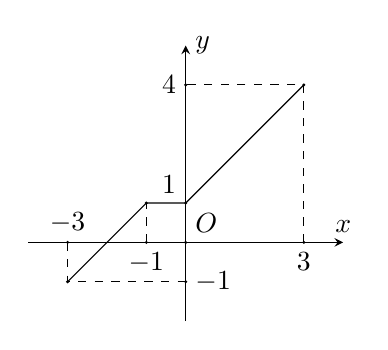
\begin{tikzpicture}[>=stealth,scale=0.5]
        \draw[->](-4,0)--(4,0)node[above]{$x$};
        \draw[->](0,-2)--(0,5)node[right]{$y$};
        \draw (-3,-1)--(-1,1)--(0,1)node[above left]{$1$}--(3,4);
        \draw[dashed](-3,0)node[above]{$-3$}--(-3,-1)--(0,-1)node[right]{$-1$};
        \draw[dashed](-1,0)node[below]{$-1$}--(-1,1);
        \draw[dashed](3,0)node[below]{$3$}--(3,4)--(0,4)node[left]{$4$};
        \fill (-3,0)circle(1.2pt) (-3,-1)circle(1.2pt) (0,-1)circle(1.2pt) (-1,0)circle(1.2pt) (-1,1)circle(1.2pt) (0,1)circle(1.2pt) (3,0)circle(1.2pt) (3,4)circle(1.2pt) (0,4)circle(1.2pt) (0,0)node[above right]{$O$}circle(1.2pt);
        \end{tikzpicture}}  
    \loigiai{
        Trên khoảng $\left(-3;-1\right)$ và $\left(1;3\right)$ đồ thị hàm số đi lên từ trái sang phải\\
        $\Rightarrow $ Hàm số đồng biến trên khoảng $\left(-3;-1\right)$ và $\left(1;3\right).$}
\end{ex}

\begin{ex}%[Phan Anh]%[0D2B1-2]
    Tìm tập xác định $\mathscr{D}$ của hàm số $y=\dfrac{\sqrt{2-x}+\sqrt{x+2}}{x}$.
    \choice
    {$\mathscr{D}=[-2;2]$}
    {$\mathscr{D}=(-2;2)\setminus\left\{0\right\}$}
    {\True $\mathscr{D}=[-2;2]\setminus\left\{0\right\}$}
    {$\mathscr{D}=\mathbb{R}$}
    \loigiai{
        Hàm số xác định khi $\heva{
            & 2-x\ge 0 \\ 
            & x+2\ge 0 \\ 
            & x\ne 0}\Leftrightarrow \heva{
            & x\le 2 \\ 
            & x\ge-2 \\ 
            & x\ne 0.}$\\
        Vậy tập xác định của hàm số là $\mathscr{D}=\left[-2;2\right]\setminus\left\{0\right\}$.}
\end{ex}

\begin{ex}%[Phan Anh]%[0D2B1-4]
    Cho hàm số $f(x)=\heva{&-x^3-6 &;x\le-2 \\&\left| x\right|&;-2<x<2 \\&x^3-6 &;x\ge 2}$. Khẳng định nào sau đây đúng?
    \choice
    {$f(x)$ là hàm số lẻ}
    {\True $f(x)$ là hàm số chẵn}
    {Đồ thị của hàm số $f(x)$ đối xứng qua gốc tọa độ}
    {Đồ thị của hàm số $f(x)$ đối xứng qua trục hoành}
    \loigiai{
        Tập xác định $\mathscr{D}=\mathbb{R}$ nên $\forall x\in\mathscr{D}\Rightarrow-x\in\mathscr{D}$.\\
        Ta có $f\left(-x\right)=\heva{&-\left(-x\right)^3-6 &; \left(-x\right)\le-2 \\&\left|-x\right| &; -2<-x<2 \\&(-x)^3-6&;\left(-x\right)\ge 2}=\heva{&x^3-6 &; x\ge 2 \\&\left| x\right| &; -2<x<2 \\&-x^3-6 &; x\le-2}=f(x)$.\\
        Vậy hàm số đã cho là hàm số chẵn.}
\end{ex}

\begin{ex}%[Phan Anh]%[0D2B1-4]
    Trong các hàm số $y=\left| x+2\right|-\left| x-2\right|$, $y=\left| 2x+1\right|+\sqrt{4x^2-4x+1}$, $y=x\left(\left| x\right|-2\right)$, $y=\dfrac{|x+2015|+|x-2015|}{|x+2015|-|x-2015|}$ có bao nhiêu hàm số lẻ?
    \choice
    {$1$}
    {$2$}
    {\True $3$}
    {$4$}
    \loigiai{\begin{itemize}
            \item Xét $f(x)=\left| x+2\right|-\left| x-2\right|$ có $\mathscr{D}=\mathbb{R}$ nên $\forall x\in\mathscr{D}\Rightarrow-x\in\mathscr{D}$.\\
            Ta có $\begin{aligned}[t]
            f(-x)&=|(-x)+2|-|(-x)-2|=|-x+2|-|-x-2|\\
            &=|x-2|-|x+2|=-(|x+2|-|x-2|)=-f(x).
            \end{aligned}$\\
            $\Rightarrow f(x)$ là hàm số lẻ.
            \item Xét $f(x)=\left| 2x+1\right|+\sqrt{4x^2-4x+1}=\left| 2x+1\right|+\sqrt{{\left(2x-1\right)}^2}=\left| 2x+1\right|+\left| 2x-1\right|$.\\
            $\mathscr{D}=\mathbb{R}$ nên $\forall x\in\mathscr{D}\Rightarrow-x\in\mathscr{D}$.\\
            Ta có $\begin{aligned}[t]
            f\left(-x\right)&=\left| 2\left(-x\right)+1\right|+\left| 2\left(-x\right)-1\right|=\left|-2x+1\right|+\left|-2x-1\right|\\
            &=\left| 2x-1\right|+\left| 2x+1\right|=\left| 2x+1\right|+\left| 2x-1\right|=f(x).
            \end{aligned}$\\
            $\Rightarrow f(x)$ là hàm số chẵn.
            \item Xét $f(x)=x\left(\left| x\right|-2\right)$ có  $\mathscr{D}=\mathbb{R}$ nên $\forall x\in\mathscr{D}\Rightarrow-x\in\mathscr{D}$.\\
            Ta có $f\left(-x\right)=\left(-x\right)\left(\left|-x\right|-2\right)=-x\left(\left| x\right|-2\right)=-f(x)\Rightarrow f(x)$ là hàm số lẻ.
            \item Xét $f(x)=\dfrac{|x+2015|+|x-2015|}{|x+2015|-|x-2015|}$ có $\mathscr{D}=\mathbb{R}\setminus\left\{0\right\}$ nên $\forall x\in\mathscr{D}\Rightarrow-x\in\mathscr{D}$.
            \\
            Ta có $\begin{aligned}[t]
            f\left(-x\right)&=\dfrac{|-x+2015|+|-x-2015|}{|-x+2015|-|-x-2015|}=\dfrac{|x-2015|+|x+2015|}{|x-2015|-|x+2015|}\\
            &=-\dfrac{|x+2015|+|x-2015|}{|x+2015|-|x-2015|}=-f(x).
            \end{aligned}$\\
            $\Rightarrow f(x)$ là hàm số lẻ.\\
            Vậy có tất cả 3 hàm số lẻ.
        \end{itemize}}
\end{ex}

\begin{ex}%[Phan Anh]%[0D2B1-2]
    Tìm tập xác định $\mathscr{D}$ của hàm số $y=\dfrac{\sqrt{x+1}}{x^2-x-6}$.
    \choice
    {$\mathscr{D}=\left\{3\right\}$}
    {\True $\mathscr{D}=\left[-1;+\infty \right)\setminus\left\{3\right\}$}
    {$\mathscr{D}=\mathbb{R}$}
    {$\mathscr{D}=\left[-1;+\infty \right)$}
    \loigiai{
        Hàm số xác định khi $\heva{
            & x+1\ge 0 \\ 
            & x^2-x-6\ne 0}\Leftrightarrow \heva{
            & x\ge-1 \\ 
            & x\ne 3 \\ 
            & x\ne-2}\Leftrightarrow \heva{
            & x\ge-1 \\ 
            & x\ne 3.}$\\
        Vậy tập xác định của hàm số là $\mathscr{D}=[-1;+\infty)\setminus\left\{3\right\}$.}
\end{ex}

\begin{ex}%[Phan Anh]%[0D2B1-2]
    Tìm tập xác định $\mathscr{D}$ của hàm số $y=\dfrac{2x+1}{x^3-3x+2}$.
    \choice
    {$\mathscr{D}=\mathbb{R}\setminus\left\{1;2\right\}$}
    {\True $\mathscr{D}=\mathbb{R}\setminus\left\{-2;1\right\}$}
    {$\mathscr{D}=\mathbb{R}\setminus\left\{-2\right\}$}
    {$\mathscr{D}=\mathbb{R}$}
    \loigiai{
        Hàm số xác định khi $\begin{aligned}[t]
        &x^3-3x+2\ne 0\Leftrightarrow (x-1)(x^2+x-2)\ne 0\\
        \Leftrightarrow&\,\heva{
            & x-1\ne 0 \\ 
            & x^2+x-2\ne 0}\Leftrightarrow \heva{
            & x\ne 1 \\ 
            & \heva{
                & x\ne 1 \\ 
                & x\ne-2}}\Leftrightarrow \heva{
            & x\ne 1 \\ 
            & x\ne-2.}
        \end{aligned}$\\
        Vậy tập xác định của hàm số là $\mathscr{D}=\mathbb{R}\setminus\left\{-2;1\right\}$.}
\end{ex}

\begin{ex}%[Phan Anh]%[0D2B1-4]
    Trong các hàm số $y=2015x$, $y=2015x+2$, $y=3x^2-1$, $y=2x^3-3x$ có bao nhiêu hàm số lẻ?
    \choice
    {$1$}
    {\True $2$}
    {$3$}
    {$4$}
    \loigiai{\begin{itemize}
            \item Xét $f(x)=2015x $ có $\mathscr{D}=\mathbb{R}$ nên $\forall x\in\mathscr{D}\Rightarrow-x\in\mathscr{D}$.\\
            Ta có $f\left(-x\right)=2015\left(-x\right)=-2015x=-f(x)\Rightarrow f(x)$ là hàm số lẻ.
            \item Xét $f(x)=2015x+2$ có $\mathscr{D}=\mathbb{R}$ nên $\forall x\in\mathscr{D}\Rightarrow-x\in\mathscr{D}$.\\
            Ta có $f\left(-x\right)=2015\left(-x\right)+2=-2015x+2\ne \pm f(x)\Rightarrow f(x)$ không chẵn, không lẻ.
            \item Xét $f(x)=3x^2-1$ có $\mathscr{D}=\mathbb{R}$ nên $\forall x\in\mathscr{D}\Rightarrow-x\in\mathscr{D}$.\\
            Ta có $f\left(-x\right)=3{\left(-x\right)}^2-1=3x^2-1=f(x)\Rightarrow f(x)$ là hàm số chẵn.
            \item Xét $f(x)=2x^3-3x$ có $\mathscr{D}=\mathbb{R}$ nên $\forall x\in\mathscr{D}\Rightarrow-x\in\mathscr{D}$.\\
            Ta có $f\left(-x\right)=2{\left(-x\right)}^3-3\left(-x\right)=-2x^3+3x=-f(x)\Rightarrow f(x)$ là hàm số lẻ.
        \end{itemize}
        Vậy có hai hàm số lẻ.}
\end{ex}

\begin{ex}%[Phan Anh]%[0D2K1-2]
    Tìm tập xác định $\mathscr{D}$ của hàm số $y=\dfrac{\sqrt{5-3\left| x\right|}}{x^2+4x+3}$.
    \choice
    {\True $\mathscr{D}=\left[-\dfrac{5}{3};\dfrac{5}{3}\right]\setminus\left\{-1\right\}$}
    {$\mathscr{D}=\mathbb{R}$}
    {$\mathscr{D}=\left(-\dfrac{5}{3};\dfrac{5}{3}\right)\setminus\left\{-1\right\}$}
    {$\mathscr{D}=\left[-\dfrac{5}{3};\dfrac{5}{3}\right]$}
    \loigiai{
        Hàm số xác định khi $\heva{
            & 5-3\left| x\right|\ge 0 \\ 
            & x^2+4x+3\ne 0}\Leftrightarrow \heva{
            & \left| x\right|\le \dfrac{5}{3} \\ 
            & x\ne-1 \\ 
            & x\ne-3}\Leftrightarrow \heva{
            &-\dfrac{5}{3}\le x\le \dfrac{5}{3} \\ 
            & x\ne-1 \\ 
            & x\ne-3}\Leftrightarrow \heva{
            &-\dfrac{5}{3}\le x\le \dfrac{5}{3} \\ 
            & x\ne-1.}$\\
        Vậy tập xác định của hàm số là $\mathscr{D}=\left[-\dfrac{5}{3};\dfrac{5}{3}\right]\setminus\left\{-1\right\}$.}
\end{ex}

\begin{ex}%[Phan Anh]%[0D2B1-4]
    Cho hàm số $f(x)=\left| x-2\right|.$ Khẳng định nào sau đây là đúng.
    \choice
    {$f(x)$ là hàm số lẻ}
    {$f(x)$ là hàm số chẵn}
    {$f(x)$ là hàm số vừa chẵn, vừa lẻ}
    {\True $f(x)$ là hàm số không chẵn, không lẻ}
    \loigiai{
        Tập xác định: $\mathscr{D}=\mathbb{R}$ nên $\forall x\in\mathscr{D}\Rightarrow-x\in\mathscr{D}$.\\
        Ta có $f\left(-x\right)=\left| \left(-x\right)-2\right|=\left| x+2\right|\ne \pm f(x)\Rightarrow f(x)$ không chẵn, không lẻ. \\
        \textbf{Lưu ý:} Hàm số vừa chẵn, vừa lẻ chỉ có một hàm duy nhất là $f(x)=0$.}
\end{ex}

\begin{ex}%[Phan Anh]%[0D2B1-3]
    Xét sự biến thiên của hàm số $f(x)=x+\dfrac{1}{x}$ trên khoảng $\left(1;+\infty \right)$. Khẳng định nào sau đây đúng?
    \choice
    {\True Hàm số đồng biến trên khoảng $\left(1;+\infty \right)$}
    {Hàm số nghịch biến trên khoảng $\left(1;+\infty \right)$}
    {Hàm số vừa đồng biến, vừa nghịch biến trên khoảng $\left(1;+\infty \right)$}
    {Hàm số không đồng biến, cũng không nghịch biến trên khoảng $\left(1;+\infty \right)$}
    \loigiai{
        Ta có
        $f\left(x_1\right)-f\left(x_2\right)=\left(x_1+\dfrac{1}{x_1}\right)-\left(x_2+\dfrac{1}{x_2}\right)=\left(x_1-x_2\right)+\left(\dfrac{1}{x_1}-\dfrac{1}{x_2}\right)=\left(x_1-x_2\right)\left(1-\dfrac{1}{x_1x_2}\right).$\\
        Với mọi $x_1, x_2\in \left(1;+\infty \right)$ và $x_1<x_2$. Ta có $\heva{
            & x_1>1 \\ 
            & x_2>1 \\}\Rightarrow x_1\cdot x_2>1\Rightarrow \dfrac{1}{x_1\cdot x_2}<1.$\\
        Suy ra $\dfrac{f\left(x_1\right)-f\left(x_2\right)}{x_1-x_2}=1-\dfrac{1}{x_1x_2}>0\Rightarrow f(x)$ đồng biến trên $\left(1;+\infty \right)$.}
\end{ex}

\begin{ex}%[Phan Anh]%[0D2B1-2]
    Tìm tập xác định $\mathscr{D}$ của hàm số $y=\dfrac{3x-1}{2x-2}$.
    \choice
    {$\mathscr{D}=\mathbb{R}$}
    {$\mathscr{D}=(1;+\infty)$}
    {\True $\mathscr{D}=\mathbb{R}\setminus\{1\}$}
    {$\mathscr{D}=[1;+\infty)$}
    \loigiai{
        Hàm số xác định khi $2x-2\ne0\Leftrightarrow x\ne1$.\\
        Vậy tập xác định của hàm số là $\mathscr{D}=\mathbb{R}\setminus\{1\}$.}
\end{ex}

\begin{ex}%[Phan Anh]%[0D2B1-2]
    Tìm tập xác định $\mathscr{D}$ của hàm số $y=\dfrac{x}{x-\sqrt{x}-6}$.
    \choice
    {$\mathscr{D}=\left[0;+\infty \right)\setminus\left\{3\right\}$}
    {\True $\mathscr{D}=\left[0;+\infty \right)\setminus\left\{9\right\}$}
    {$\mathscr{D}=\left[0;+\infty \right)\setminus\left\{\sqrt{3}\right\}$}
    {$\mathscr{D}=\mathbb{R}\setminus\left\{9\right\}$}
    \loigiai{
        Hàm số xác định khi $\heva{
            & x\ge 0 \\ 
            & x-\sqrt{x}-6\ne 0}\Leftrightarrow \heva{
            & x\ge 0 \\ 
            & \sqrt{x}\ne 3}\Leftrightarrow \heva{
            & x\ge 0 \\ 
            & x\ne 9.}$\\
        Vậy tập xác định của hàm số là $\mathscr{D}=\left[0;+\infty \right)\setminus\left\{9\right\}$.}
\end{ex}

\begin{ex}%[Phan Anh]%[0D2B1-2]
    Tìm tập xác định $\mathscr{D}$ của hàm số $y=\dfrac{x+1}{(x+1)(x^2+3x+4)}$.
    \choice
    {$\mathscr{D}=\mathbb{R}\setminus\left\{1\right\}$}
    {$\mathscr{D}=\left\{-1\right\}$}
    {\True $\mathscr{D}=\mathbb{R}\setminus\left\{-1\right\}$}
    {$\mathscr{D}=\mathbb{R}$}
    \loigiai{
        Hàm số xác định khi $\heva{
            & x+1\ne 0 \\ 
            & x^2+3x+4\ne 0}\Leftrightarrow x\ne-1$.\\
        Vậy tập xác định của hàm số là $\mathscr{D}=\mathbb{R}\setminus\left\{-1\right\}$.}
\end{ex}

\begin{ex}%[Phan Anh]%[0D2B1-2]
    Tìm tập xác định $\mathscr{D}$ của hàm số $y=\dfrac{2018}{\sqrt[3]{x^2-3x+2}-\sqrt[3]{x^2-7}}$.
    \choice
    {\True $\mathscr{D}=\mathbb{R}\setminus\left\{3\right\}$}
    {$\mathscr{D}=\mathbb{R}$}
    {$\mathscr{D}=\left(-\infty;1\right)\cup \left(2;+\infty \right)$}
    {$\mathscr{D}=\mathbb{R}\setminus\left\{0\right\}$}
    \loigiai{
        Hàm số xác định khi $\begin{aligned}[t]
        &\sqrt[3]{x^2-3x+2}-\sqrt[3]{x^2-7}\ne 0\Leftrightarrow \sqrt[3]{x^2-3x+2}\ne \sqrt[3]{x^2-7}\\
        \Leftrightarrow&\,x^2-3x+2\ne x^2-7\Leftrightarrow 9\ne 3x\Leftrightarrow x\ne 3.
        \end{aligned}$\\
        Vậy tập xác định của hàm số là $\mathscr{D}=\mathbb{R}\setminus\left\{3\right\}$.}
\end{ex}

\begin{ex}%[Phan Anh]%[0D2B1-2]
    Tìm tập xác định $\mathscr{D}$ của hàm số $y=\sqrt{x+2}-\sqrt{x+3}$.
    \choice
    {$\mathscr{D}=[-3;+\infty)$}
    {\True $\mathscr{D}=\left[-2;+\infty \right)$}
    {$\mathscr{D}=\mathbb{R}$}
    {$\mathscr{D}=\left[2;+\infty \right)$}
    \loigiai{
        Hàm số xác định khi $\heva{
            & x+2\ge 0 \\ 
            & x+3\ge 0 \\}\Leftrightarrow \heva{
            & x\ge-2 \\ 
            & x\ge-3 \\}\Leftrightarrow x\ge-2$.\\
        Vậy tập xác định của hàm số là $\mathscr{D}=\left[-2;+\infty \right)$.}
\end{ex}

\begin{ex}%[Phan Anh]%[0D2B2-2]
    Tìm $a$ và $b$ để đồ thị hàm số $y=ax+b$ đi qua các điểm $A(-2;1)$, $B(1;-2)$.
    \choice
    {$a=-2$ và $b=-1$}
    {$a=2$ và $b=1$}
    {$a=1$ và $b=1$}
    {\True $a=-1$ và $b=-1$}
    \loigiai{
        Đồ thị hàm số đi qua các điểm $A(-2;1)$, $B(1;-2)$ nên
        $\heva{& 1=a\times(-2)+b \\ 
            &-2=a\times1+b}\Leftrightarrow \heva{
            & a=-1 \\ 
            & b=-1.}$}
\end{ex}

\begin{ex}%[Phan Anh]%[0D2B2-2]
    Biết rằng đồ thị hàm số $y=ax+b$ đi qua điểm $A(-3;1)$ và có hệ số góc bằng $-2$. Tính tích $P=ab$.
    \choice
    {$P=-10$}
    {\True $P=10$}
    {$P=-7$}
    {$P=-5$}
    \loigiai{
        Hệ số góc bằng $-2\Rightarrow a=-2$.
        Đồ thị đi qua điểm $A(-3;1)\Rightarrow-3a+b=1\Rightarrow b=-5$.\\
        Vậy $P=ab=(-2)\times(-5)=10$.}
\end{ex}

\begin{ex}%[Phan Anh]%[0D2K2-4]
Tìm giá trị thực của tham số $m$ để ba đường thẳng $y=2x$, $y=-x-3$ và $y=mx+5$ phân biệt và đồng qui.
\choice
{$m=-7$}
{$m=5$}
{$m=-5$}
{\True $m=7$}
\loigiai{
    Tọa độ giao điểm $A$ của hai đường thẳng $y=2x$ và $y=-x-3$ là nghiệm của hệ\\ $\heva{
        & y=2x \\ 
        & y=-x-3}\Leftrightarrow \heva{
        & x=-1 \\ 
        & y=-2}\Rightarrow A(-1;-2)$.\\
    Để ba đường thẳng đồng quy thì đường thẳng $y=mx+5$ đi qua $A$
    $\Rightarrow-2=-1\times m+5\Rightarrow m=7$.\\
    Thử lại, với $m=7$ thì ba đường thẳng $y=2x$; $y=-x-3$ ; $y=7x+5$ phân biệt và đồng quy.}
\end{ex}

\begin{ex}%[Phan Anh]%[0D2B2-3]
    Đồ thị hình vẽ là đồ thị của một hàm số trong bốn hàm số được liệt kê ở bốn phương án A, B, C, D dưới đây.
    Hỏi hàm số đó là hàm số nào?
    \begin{center}
        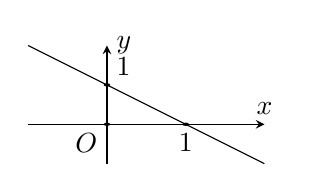
\begin{tikzpicture}[>=stealth,yscale=0.5]
        \draw[->](-1,0)--(2,0)node[above]{$x$};
        \draw[->](0,-1)--(0,2)node[right]{$y$};
        \draw[smooth,samples=100,domain=-1:2]plot(\x,{-\x+1});
        \fill (0,1)node[above right]{$1$}circle(1.2pt) (1,0)node[below]{$1$}circle(1.2pt) (0,0)node[below left]{$O$}circle(1.2pt);
        \end{tikzpicture}
    \end{center}
    \choice
    {$y=x+1$}
    {$y=-x+2$}
    {$y=2x+1$}
    {\True $y=-x+1$}
    \loigiai{
        Đồ thị đi xuống từ trái sang phải $\Rightarrow$ hệ số góc $a<0$.\\
        Đồ thị hàm số cắt trục tung tại điểm $\left(0;1\right)$.\\
        Do đó, hàm số $y=-x+1$ thỏa bài toán.}
\end{ex}

\begin{ex}%[Phan Anh]%[0D2B2-1]
    Tìm tất cả các giá trị thực của tham số $m$ để đường thẳng $y=\left(m^2-3\right)x+2m-3$ song song với đường thẳng $y=x+1$.
    \choice
    {$m=2$}
    {$m=\pm 2$}
    {\True $m=-2$.}
    {$m=1$}
    \loigiai{Đường thẳng $y=\left(m^2-3\right)x+2m-3$ song song với đường thẳng $y=x+1$ khi và chỉ khi $$\heva{
            & m^2-3=1 \\ 
            & 2m-3\ne 1}\Leftrightarrow \heva{
            & m=\pm 2 \\ 
            & m\ne 2}\Leftrightarrow m=-2.$$}
\end{ex}

\begin{ex}%[Phan Anh]%[0D2B2-4]
Cho hàm số bậc nhất $y=ax+b$. Tìm $a$ và $b$, biết rằng đồ thị hàm số đi qua điểm $M(-1;1)$ và cắt trục hoành tại điểm có hoành độ là 5.
\choice
{$a=\dfrac{1}{6}$; $b=\dfrac{5}{6}$}
{$a=-\dfrac{1}{6}$; $b=-\dfrac{5}{6}$}
{$a=\dfrac{1}{6}$; $b=-\dfrac{5}{6}$}
{\True $a=-\dfrac{1}{6}$; $b=\dfrac{5}{6}$}
\loigiai{
    Đồ thị hàm số đi qua điểm $M(-1;1)\Rightarrow1=a\times(-1)+b.\quad(1)$
    \\
    Đồ thị hàm số cắt trục hoành tại điểm có hoành độ là $5\Rightarrow0=a\times5+b$.\quad$(2)$
    \\
    Từ $(1)$ và $(2)$, ta có hệ $\heva{
        & 1=a\times(-1)+b \\ 
        & 0=a\times5+b}\Leftrightarrow \heva{
        &-a+b=1 \\ 
        & 5a+b=0}\Leftrightarrow \heva{
        & a=-\dfrac{1}{6} \\ 
        & b=\dfrac{5}{6}.}$}
\end{ex}

\begin{ex}%[Phan Anh]%[0D2B2-1]
    Tìm $m$ để hàm số $y=m(x+2)-x(2m+1)$ nghịch biến trên $\mathbb{R}$.
    \choice
    {$m>-2$}
    {$m<-\dfrac{1}{2}$}
    {\True $m>-1$}
    {$m>-\dfrac{1}{2}$}
    \loigiai{
        Viết lại $y=m(x+2)-x(2m+1)=(-1-m)x+2m$.\\
        Hàm số bậc nhất $y=ax+b$ nghịch biến khi $a<0$ nên suy ra $-1-m<0\Leftrightarrow m>-1$.}
\end{ex}

\begin{ex}%[Phan Anh]%[0D2B2-4]
    Tìm giá trị thực của $m$ để hai đường thẳng $d\colon y=mx-3$ và $\Delta\colon y+x=m$ cắt nhau tại một điểm nằm trên trục tung.
    \choice
    {\True $m=-3$}
    {$m=3$}
    {$m=\pm 3$}
    {$m=0$}
    \loigiai{
        Gọi $A(0;a)$ là giao điểm hai đường thẳng nằm trên trục tung.\\
        $\Rightarrow\heva{
            & A\in d \\ 
            & A\in \Delta}\Rightarrow\heva{
            & a=0\times m-3 \\ 
            & a+0=m}\Leftrightarrow\heva{
            & a=-3 \\ 
            & m=-3.}$}
\end{ex}

\begin{ex}%[Phan Anh]%[0D2B2-1]
    Tìm tất cả các giá trị thực của tham số $m$ để đường thẳng $d\colon y=(3m+2)x-7m-1$ vuông góc với đường $\Delta\colon y=2x-1$.
    \choice
    {$m=0$}
    {\True $m=-\dfrac{5}{6}$}
    {$m<\dfrac{5}{6}$}
    {$m>-\dfrac{1}{2}$}
    \loigiai{Đường thẳng $\Delta $ vuông góc với đường thẳng $d$ khi và chỉ khi $2(3m+2)=-1\Leftrightarrow m=-\dfrac{5}{6}$.}
\end{ex}

\begin{ex}%[Phan Anh]%[0D2K2-4]
Cho hàm số bậc nhất $y=ax+b$. Tìm $a$ và $b$, biết rằng đồ thị hàm số cắt đường thẳng $\Delta_1:y=2x+5$ tại điểm có hoành độ bằng $-2$ và cắt đường thẳng $\Delta_2:y=-3x+4$ tại điểm có tung độ bằng $-2$.
\choice
{$a=\dfrac{3}{4}$; $b=\dfrac{1}{2}$}
{$a=-\dfrac{3}{4}$; $b=\dfrac{1}{2}$}
{\True $a=-\dfrac{3}{4}$; $b=-\dfrac{1}{2}$}
{$a=\dfrac{3}{4}$; $b=-\dfrac{1}{2}$}
\loigiai{
    Với $x=-2$ thay vào $y=2x+5$, ta được $y=1$.\\
    Đồ thị hàm số cắt đường thẳng $\Delta_1$ tại điểm có hoành độ bằng $-2$ nên đi qua điểm $A(-2;1)$.\\
    Do đó ta có $1=a\times(-2)+b.\quad(1)$\\
    Với $y=-2$ thay vào $y=-3x+4$, ta được $x=2$.\\
    Đồ thị hàm số cắt đường thẳng $y=-3x+4$ tại điểm có tung độ bằng $-2$ nên đi qua điểm $B(2;-2)$.\\
    Do đó ta có $-2=a\times2+b.\quad(2)$\\
    Từ $(1)$ và $(2)$, ta có hệ $\heva{
        & 1=a\times(-2)+b \\ 
        &-2=a\times2+b}\Leftrightarrow \heva{
        &-2a+b=1 \\ 
        & 2a+b=-2}\Leftrightarrow \heva{
        & a=-\dfrac{3}{4} \\ 
        & b=-\dfrac{1}{2}.}$}
\end{ex}

\begin{ex}%[Phan Anh]%[0D2B2-3]
    \immini{Đồ thị hình vẽ là đồ thị của một hàm số trong bốn hàm số được liệt kê ở bốn phương án A, B, C, D dưới đây.
    Hỏi hàm số đó là hàm số nào?
    \choice
    {$y=|x|+1$}
    {\True $y=2|x|+1$}
    {$y=|2x+1|$}
    {$y=|x+1|$}}{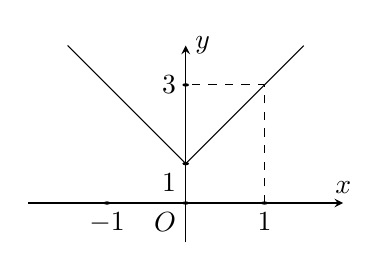
\begin{tikzpicture}[>=stealth,yscale=0.5]
    \draw[->](-2,0)--(2,0)node[above]{$x$};
    \draw[->](0,-1)--(0,4)node[right]{$y$};
    \draw[smooth,samples=100,domain=0:1.5]plot(\x,{2*\x+1});
    \draw[smooth,samples=100,domain=-1.5:0]plot(\x,{-2*\x+1});
    \draw[dashed](1,0)node[below]{$1$}--(1,3)--(0,3)node[left]{$3$};
    \fill (-1,0)node[below]{$-1$} circle(1.2pt) (0,0)node[below left]{$O$}circle(1.2pt) (0,1)node[below left]{$1$} circle (1.2pt) (1,0) circle(1.2pt) (0,3)circle(1.2pt);
    \end{tikzpicture}}
    \loigiai{
        Đồ thị hàm số đi qua điểm $(1;3)$.\\
        Đồ thị hàm số không có điểm chung với trục hoành. Nên nhận hàm số $y=2|x|+1$.}
\end{ex}

\begin{ex}%[Phan Anh]%[0D2K2-4]
Đường thẳng $d\colon \dfrac{x}{a}+\dfrac{y}{b}=1$, $a\ne0$; $b\ne0$ đi qua điểm $M(-1;6)$ tạo với các tia $Ox$, $Oy$ một tam giác có diện tích bằng $4$. Tính $S=a+2b$.
\choice
{$S=-\dfrac{38}{3}$}
{$S=\dfrac{-5+7\sqrt{7}}{3}$}
{\True $S=10$}
{$S=6$}
\loigiai{
    Đường thẳng $d\colon \dfrac{x}{a}+\dfrac{y}{b}=1$ đi qua điểm $M(-1;6)\Rightarrow\dfrac{-1}{a}+\dfrac{6}{b}=1.\quad(1)$\\
    Ta có $d\cap Ox=A(a;0)$; $d\cap Oy=B(0;b)$.\\
    Suy ra $OA=|a|=a$ và $OB=|b|=b$ (do $A$, $B$ thuộc hai tia $Ox$, $Oy$).\\
    Tam giác $OAB$ vuông tại $O$. Do đó, ta có $S_{\triangle ABC}=\dfrac{1}{2}OA\times OB=4\Rightarrow\dfrac{1}{2}ab=4.\quad(2)$\\
    Từ $(1)$ và $(2)$ ta có hệ
    $\heva{&-\dfrac{1}{a}+\dfrac{6}{b}=1 \\ 
        & \dfrac{1}{2}ab=4}\Leftrightarrow \heva{
        & 6a-b-ab=0 \\ 
        & ab=8}\\\Leftrightarrow \heva{
        & 6a-b-8=0 \\ 
        & ab=8}\Leftrightarrow \heva{
        & b=6a-8 \\ 
        & a(6a-8)-8=0}\Leftrightarrow \heva{
        & b=6a-8 \\ 
        & \hoac{
            & a=2 \\ 
            & a=-\dfrac{2}{3}.}}$\\
    Do $A$ thuộc tia $Ox$ $\Rightarrow a=2$. Khi đó, $b=6a-8=4$. Suy ra $a+2b=10$.}
\end{ex}

\begin{ex}%[Phan Anh]%[0D2B2-3]
    \immini{Đồ thị hình bên là đồ thị của một hàm số trong bốn hàm số được liệt kê ở bốn phương án A, B, C, D dưới đây. Hỏi hàm số đó là hàm số nào?
    \choice
    {$y=\left| x\right|$}
    {$y=\left| x\right|+1$}
    {\True $y=1-\left| x\right|$}
    {$y=\left| x\right|-1$}}{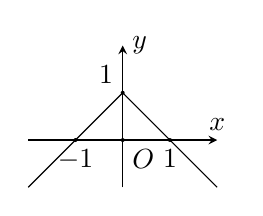
\begin{tikzpicture}[>=stealth,scale=0.6]
    \draw[->](-2,0)--(2,0)node[above]{$x$};
    \draw[->](0,-1)--(0,2)node[right]{$y$};
    \draw[smooth,samples=100,domain=-2:0]plot(\x,{1+\x});
    \draw[smooth,samples=100,domain=0:2]plot(\x,{1-\x});
    \fill (0,1)node[above left]{$1$}circle(1.2pt) (-1,0)node[below]{$-1$}circle(1.2pt) (0,0)node[below right]{$O$}circle(1.2pt) (1,0)node[below]{$1$}circle(1.2pt);
    \end{tikzpicture}}
    \loigiai{
        Giao điểm của đồ thị hàm số với trục tung là $\left(0;1\right)$.\\
        Giao điểm của đồ thị hàm số với trục hoành là $(-1;0)$ và $(1;0)$. Nên nhận hàm số $y=1-\left| x\right|$.}
\end{ex}

\begin{ex}%[Phan Anh]%[0D2B2-2]
    Biết rằng đồ thị hàm số $y=ax+b$ đi qua điểm $N(4;-1)$ và vuông góc với đường thẳng $4x-y+1=0$. Tính tích $P=ab$.
    \choice
    {\True $P=0$}
    {$P=-\dfrac{1}{4}$}
    {$P=\dfrac{1}{4}$}
    {$P=-\dfrac{1}{2}$}
    \loigiai{
        Đồ thị hàm số đi qua điểm $N(4;-1)$ nên $-1=a\times4+b.\quad(1)$\\
        Mặt khác, đồ thị hàm số vuông góc với đường thẳng $y=4x+1$ nên $4\times a=-1.\quad(2)$\\
        Từ $(1)$ và $(2)$, ta có hệ $\heva{
            &-1=a\times4+b \\ 
            & 4a=-1}\Leftrightarrow \heva{
            & a=-\dfrac{1}{4} \\ 
            & b=0}\Rightarrow P=ab=0$.}
\end{ex}

\begin{ex}%[Phan Anh]%[0D2B2-1]
    Biết rằng đồ thị hàm số $y=ax+b$ đi qua điểm $E(2;-1)$ và song song với đường thẳng $ON$ với $O$ là gốc tọa độ và $N(1;3)$. Tính giá trị biểu thức $S=a^2+b^2$.
    \choice
    {$S=-4$}
    {$S=-40$}
    {$S=-58$}
    {\True $S=58$}
    \loigiai{
        Đồ thị hàm số đi qua điểm $E\left(2;-1\right)$ nên $-1=a\times2+b.\quad(1)$\\
        Gọi $y=a'x+b'$ là đường thẳng đi qua hai điểm $O(0;0)$ và $N(1;3)$ nên
        $\heva{
            & 0=a'\times0+b'\\ 
            & 3=a'\times1+b'}\Leftrightarrow \heva{
            & a'=3 \\ 
            & b'=0.}$\\
        Đồ thị hàm số song song với đường thẳng $ON$ nên $\heva{
            & a=a'=3 \\ 
            & b\ne b'=0.}\quad(2)$\\
        Từ $(1)$ và $(2)$, ta có hệ $\heva{
            &-1=a\cdot2+b \\ 
            & a=3}\Leftrightarrow \heva{
            & a=3 \\ 
            & b=-7}\Rightarrow S=a^2+b^2=58$.}
\end{ex}

\begin{ex}%[Phan Anh]%[0D2B2-1]
    Biết rằng đồ thị hàm số $y=ax+b$ đi qua điểm $M(1;4)$ và song song với đường thẳng $y=2x+1$. Tính tổng $S=a+b$.
    \choice
    {\True $S=4$}
    {$S=2$}
    {$S=0$}
    {$S=-4$}
    \loigiai{Đồ thị hàm số đi qua điểm $M(1;4)$ nên $4=a\times 1+b.\quad(1)$\\
        Mặt khác, đồ thị hàm số song song với đường thẳng $y=2x+1$ nên $\heva{
            & a=2 \\ 
            & b\ne 1.}\quad(2)$\\
        Từ $(1)$ và $(2)$, ta có hệ $\heva{
            & 4=a\times1+b \\ 
            & a=2}\Leftrightarrow \heva{
            & a=2 \\ 
            & b=2}\Rightarrow a+b=4$.}
\end{ex}

\begin{ex}%[Phan Anh]%[0D2K2-1]
    Có bao nhiêu giá trị nguyên của tham số $m$ thuộc đoạn $[-2017;2017]$ để hàm số $y=\left(m^2-4\right)x+2m$ đồng biến trên $\mathbb{R}$?
    \choice
    {\True $4030$}
    {$4034$}
    {Vô số}
    {$2015$}
    \loigiai{
        Hàm số bậc nhất $y=ax+b$ đồng biến khi $a>0\Leftrightarrow m^2-4>0\Leftrightarrow \hoac{
            & m>2 \\ 
            & m<-2}$\\
        $\Rightarrow m\in\{-2017;-2016;-2015;\ldots;-3\}\cup\{3;4;5;\ldots;2017\}$.\\
        Vậy có $2\times(2017-3+1)=2\times2015=4030$ giá trị nguyên của $m$ cần tìm.}
\end{ex}

\begin{ex}%[Phan Anh]%[0D2B2-3]
    \immini{Cho hàm số $y=ax+b$ có đồ thị là hình bên. Tìm $a$ và $b$.
    \choice
    {$a=-2$ và $b=3$}
    {$a=-\dfrac{3}{2}$ và $b=2$}
    {$a=-3$ và $b=3$}
    {\True $a=\dfrac{3}{2}$ và $b=3$}}{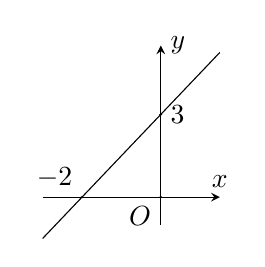
\begin{tikzpicture}[>=stealth,yscale=0.7,scale=0.5]
    \draw[->](-3,0)--(1.5,0)node[above]{$x$};
    \draw[->](0,-1)--(0,5.5)node[right]{$y$};
    \draw[smooth,samples=100,domain=-3:1.5]plot(\x,{1.5*\x+3});
    \fill (0,3)node[right]{$3$}circle(1.2pt) (-2,0)node[above left]{$-2$}circle(1.2pt) (0,0)node[below left]{$O$}circle(1.2pt);
    \end{tikzpicture}}
            \loigiai{
        Đồ thị hàm số $y=ax+b$ đi qua điểm $A\left(-2;0\right)$ suy ra $-2a+b=0.\quad(1)$\\
        Đồ thị hàm số $y=ax+b$ đi qua điểm $B\left(0;3\right)$ suy ra $b=3.\quad(2)$\\
        Từ $(1)$ và $(2)$ suy ra $\heva{
            &-2a+b=0 \\ 
            & b=3}\Leftrightarrow \heva{
            & 2a=3 \\ 
            & b=3}\Leftrightarrow \heva{
            & a=\dfrac{3}{2} \\ 
            & b=3.}$}
\end{ex}

\begin{ex}%[Phan Anh]%[0D2B2-3]
    \immini{Đồ thị hình vẽ là đồ thị của một hàm số trong bốn hàm số được liệt kê ở bốn phương án A, B, C, D dưới đây. Hỏi hàm số đó là hàm số nào?
    \choice
    {$y=\left| x\right|$}
    {$y=-x$}
    {$y=\left| x\right|$ với $x>0$}
    {\True $y=-x$ với $x<0$}}{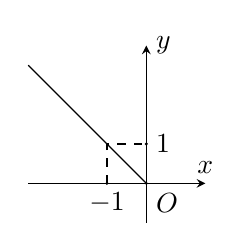
\begin{tikzpicture}[>=stealth,scale=0.5]
    \draw[->](-3,0)--(1.5,0)node[above]{$x$};
    \draw[->](0,-1)--(0,3.5)node[right]{$y$};
    \draw[smooth,samples=100,domain=-3:0]plot(\x,{-\x});
    \fill (0,1)node[right]{$1$}circle(1.2pt) (-1,0)node[below]{$-1$}circle(1.2pt) (0,0)node[below right]{$O$}circle(1.2pt);
    \draw [dashed] (-1,0)--(-1,1)--(0,1);
    \end{tikzpicture}}
    \loigiai{
        Đồ thị hàm số nằm hoàn toàn ``bên trái'' trục tung.\\
        Đồ thị hàm số đi xuống từ trái sang phải $\Rightarrow a<0$. Nên nhận hàm số $y=-x$ với $x<0$.}
\end{ex}

\begin{ex}%[Phan Anh]%[0D2K2-4]
Tìm phương trình đường thẳng $d\colon y=ax+b$. Biết đường thẳng $d$ đi qua điểm $I(1;2)$ và tạo với hai tia $Ox$, $Oy$ một tam giác có diện tích bằng $4$.
\choice
{$y=-2x-4$}
{\True $y=-2x+4$}
{$y=2x-4$}
{$y=2x+4$}
\loigiai{
    Đường thẳng $d\colon y=ax+b$ đi qua điểm $I(1;2)\Rightarrow2=a+b.\quad(1)$\\
    Ta có $d\cap Ox=A\left(-\dfrac{b}{a};0\right)$; $d\cap Oy=B(0;b)$.\\
    Suy ra $OA=\left|-\dfrac{b}{a}\right|=-\dfrac{b}{a}$ và $OB=|b|=b$ (do $A$, $B$ thuộc hai tia $Ox$, $Oy$).\\
    Tam giác $OAB$ vuông tại $O$.
    Do đó, ta có $$S_{\triangle ABC}=\dfrac{1}{2}OA\times OB=4\Rightarrow\dfrac{1}{2}\times\left(-\dfrac{b}{a}\right)\times b=4\Rightarrow b^2=-8a.\quad(2)$$
    Từ $(1)$ suy ra $b=2-a$. Thay vào $(2)$, ta được
    $$(2-a)^2=-8a\Leftrightarrow a^2-4a+4=-8a\Leftrightarrow a^2+4a+4=0\Leftrightarrow a=-2.$$
    Với $a=-2\Rightarrow b=4$. Vậy đường thẳng cần tìm là $d\colon y=-2x+4$.}
\end{ex}

\Closesolutionfile{ans}